\chapter{مقدمه}






پویانمایی هنر جان‌بخشیدن به اجسام بدون جان است.
والت دیزنی درباره‌‌ی پویانمایی می‌گوید: "پویانمایی می تواند هر آنچه را که ذهن انسان تصور می‌کند، توضیح دهد"

وقتی می‌گوییم جسمی را پویا کردیم، یعنی به آن جان بخشیدیم.
زمانی که یک فیلم پویانمایی شده را در تلوزیون یا سینما می‌بینید، شخصیت‌های درون آن فیلم در حالت حرکت هستند.
این حرکت معمولا صاف و به هم پیوسته است. نوارهای حاوی فیلم متشکل از دنباله‌ای از تصاویر هستند که به عنوان "فریم" شناخته می‌شوند و درواقع با پخش شدن این فریم‌ها
به صورت متوالی، توهم ایجاد حرکت به مخاطب ابراز می‌شود.

پویانمایی از گذشته تا امروز تغییرات فراوانی را دیده است.
در پویانمایی سنتی، تصاویر به وسیله‌‌ی دست روی صفحات سلولوئیدی شفاف ترسیم یا نقاشی شده 
سپس از آن‌ها عکس گرفته و روی فیلم نمایش داده می‌شدند.
امروزه اکثر پویانمایی‌ها با تصاویر کامپیوتری
\LTRfootnote{CGI}
ساخته می‌شوند.
\cite{AnimationWikipedia}
علاوه بر این، دامنه‌ی استفاده از این پویانمایی نیز دستخوش بسیاری تغییرات شده‌است.
در گذشته پویانمایی را می‌توانستیم در فیلم‌های پویانمایی شده یا کارتون‌ها مشاهده کنیم.
اما اکنون با پیشرفت تکنولوژی، پویانمایی نقش بسیار اساسی‌ای در بازی‌های کامپیوتری پیدا کرده است.
هدف بازی‌‌های کامپیوتری، به خصوص بازی‌های کامپیوتری داستان محور، غوطه‌ور کردن بازیکن 
در داستان است.
همانطور که اشاره شد پویانمایی هنر جان بخشیدن به اجسام است و به وسیله‌ی 
آن است که می‌توانیم احساسات و اعمال شخصیت بازی را به بازیکن منتقل کنیم.

بازی‌های کامپیوتری به صورت معمول توسط موتور‌های بازی‌سازی ساخته می‌شوند.
اگر بخواهیم تعریفی برای موتور بازی‌سازی آوریم می‌توان گفت 
آن‌ها پلتفرم‌هایی هستند که ساخت بازی‌های رایانه‌ای را آسان‌تر می‌کنند.
موتور‌های بازی‌سازی متشکل از مولفه‌های مختلفی هستند که قابلیت‌های لازم برای ساخت بازی را فراهم می‌کنند.
از رایج‌ترین مولفه‌های موتور بازی می‌توان به مولفه‌ی صدا، مولفه‌ی رندر، مولفه‌ی هوش مصنوعی و مولفه‌ی انیمیشن اشاره کرد.
\cite{barczak2019comparative}

هدف اصلی این پروژه آشنایی با روش‌های استفاده شده در محیط‌های گرافیکی مانند موتورهای بازی‌سازی با تاکید بیشتر بر 
روی سیستم‌های پویانمایی به کار رفته در این محیط‌ها است.

به همین جهت این پروژه به دو صورت این هدف را دنبال می‌کند.
جهت آشناشدن با یک موتور بازی‌سازی و نحوه‌ی پیاده‌سازی سیستم پویانمایی آن، موتور 
بازی‌سازی آنریل انتخاب شده است.
آنریل یکی از معروف ترین موتور‌های بازی‌سازی در جهان است که اولین نسل آن
توسط تیم سوینی، بنیانگذار اپیک گیمز 
\LTRfootnote{Epic Games}
، توسعه یافت.
آخرین نسخه‌ی این موتور به اسم موتور بازی‌سازی آنریل 5 
در سال 2020 معرفی و در سال 2022 انتشار یافت.
سیستم پویانمایی این موتور بسیار وسیع است. به همین دلیل بخش کوچکی از این سیستم که گراف پویانمایی نام دارد، انتخاب شده است.
بنابراین به بررسی ساختار و نحوه‌ی استفاده از این گراف می‌پردازیم.

پس از بدست آوردن تجربه‌ی اولیه از گراف انیمیشن برای آشنایی کامل تر 
با محیط گرافیکی و همچنین سیستم پویانمایی به پیاده‌سازی یک سیستم پویانمایی با استفاده از 
\lr{OpenGL}
پرداختیم.
\lr{OpenGL}
یک واسط برنامه نویسی کاربردی
\LTRfootnote{API}
است که با فراهم کردن توابع مختلف به توسعه‌دهندگان امکان دستکاری گرافیک و تصاویر را می ‌دهد.
با استفاده از این 
\lr{API}
می‌توان آشنایی خوبی در مورد گرافیک کامپیوتری و به صورت کلی محیط‌های گرافیکی بدست آورد.
برای محیط سه‌بعدی پیاده‌سازی شده از روش 
\lr{Phong Shading}
برای نورپردازی محیط استفاده شده است. این روش یکی از معروف ترین روش‌های نورپردازی در محیط‌های سه‌بعدی بلادرنگ به‌خصوص بازی‌های کامپیوتری است. علاوه بر تولید صحنه‌ی سه‌بعدی،
برای بدست آوردن آشنایی کامل با سیستم‌های پویانمایی که دربازی‌ها استفاده می‌شوند، به پیاده‌سازی یک نمونه از آن پرداختم.
در این پیاده‌سازی سیستم پویانمایی به چند بخش کلی تقسیم شده است که هر کدام هدف‌های مختلفی را دنبال می‌کند.
برای اینکه یک سیستم پویانمایی داشته باشیم در ابتدا به یک شخصیتی نیاز داریم 
تا کلیپ‌های پویانمایی بر روی آن اجرا شود.
شخصیت‌ها در این پیاده‌سازی توسط کتابخانه‌ی 
\lr{Assimp}
در ساختمان داده‌های مناسب ذخیره می‌شود.
هر شخصیت در این پیاده‌سازی به دو قسمت کلی مش و اسکلت تقسیم می‌شود.
یکی از وظایف مهم این پیاده‌سازی، اتصال این دو قسمت به یکدگیر 
است.
این اتصال به صورت کلی به اسم 
\lr{Skinning}
نام دارد. 
مرحله‌ی بعدی پیاده‌سازی به پخش کلیپ‌های پویانمایی بر روی این شخصیت می‌پردازد.
درنهایت از ماشین حالت متناهی برای برای ترکیب کلیپ‌های پویانمایی متفاوت با یکدیگر استفاده شده است.

خروجی این پروژه یک تحقیق در مورد سیستم گراف پویانمایی آنریل به همراه 
یک نرم‌افزار گرافیکی سیستم انیمیشن است.

در فصل‌های آتی به بررسی این موارد گفته‌شده پرداخته می‌شود.
ابتدا در فصل دوم یک مروری بر تاریخچه‌ی انیمیشن‌ها می‌شود. سپس توضیحاتی درباره‌ی موتور بازی‌سازی و 
موتور بازی‌سازی آنریل داده می‌شود و درنهایت توضیحاتی کلی 
درباره‌ی پویانمایی اسکلتونی که به وفور در موتور‌های بازی‌سازی استفاده می‌شود داده می‌شود.

در فصل سوم به بررسی موتور بازی‌سازی آنریل با تاکید بر روی گراف پویانمایی می‌پردازیم و نحوه‌ی استفاده از آن را بررسی می‌کنیم.

در نهایت در فصل چهارم توضیحاتی درباره‌ی نحوه‌ی پیاده‌سازی سیستم پویانمایی
به همراه توضیحات سیستم‌های موجود در این پیاده‌سازی می‌پردازیم.

در فصل "نتیجه‌گیری"، یک نتیجه‌گیری کلی از خروجی‌های این پروژه ارائه کرده 
و در فصل "کارهای آینده"، به بررسی مشکلاتی که می‌تواند در پیاده‌سازی برطرف شود به همراه 
پیشنهاداتی برای ادامه‌ی این پروژه پرداخته می‌شود.



پویانمایی تاریخچه‌ای غنی‌ دارد. در این فصل ابتدا به بررسی این تاریخچه با توضیحاتی 
درباره‌ی پویانمایی سنتی و پس از آن پویانمایی کامپیوتری پرداخته می‌شود.
پس از آن به بررسی روش‌های کلی که توسط هنرمندان برای ایجاد پویانمایی به‌کارگرفته می‌شوند پرداخته می‌شود.
در نهایت به بررسی به کارگرفتن این انیمیشن‌ها در موتورهای بازی سازی پرداخته می‌شود.




--




\section{تاریخچه‌ی پویانمایی سنتی}

پویانمایی سنتی که با اسم‌های مختلفی مانند "پویانمایی مرسوم" ، "پویانمایی سل‌ای"و "پویانمایی بادست" شناخته می‌شود، روشی 
غالب برای تولید فیلم‌های پویانمایی‌شده در حدود قرن 20 میلادی بود.
در این روش، به صورت کلی پویانمایی به وسیله‌ی نقاشی با دست به وجود می‌‌آمد.
درواقع هر فریم از فیلم، یک عکسی از نقاشی بود.
برای به وجود آوردن توهم حرکت، هر نقاشی اندکی با نقاشی قبلی خود تفاوت داشت.

برای تولید پویانمایی سنتی، از روش‌های مختلفی استفاده می‌شد. در اینجا به بررسی
سه عدد از این روش‌ها می‌پردازیم.

\subsection{فریم‌های کلیدی و درمیان}
از آنجایی که تولید پویایی با دست و کشیدن نقاشی کار بسیار طولانی‌ای بود، برای اینکه وقت پویانمای‌های ارشد 
ذخیره شود، این پویانماها فریم‌های اصلی یک حرکت را بر روی کاغذ ترسیم می‌کردند و 
فریم‌های میانی را پویانماهای جوان پر می‌کردند.

\begin{figure}[ht]
	\centerline{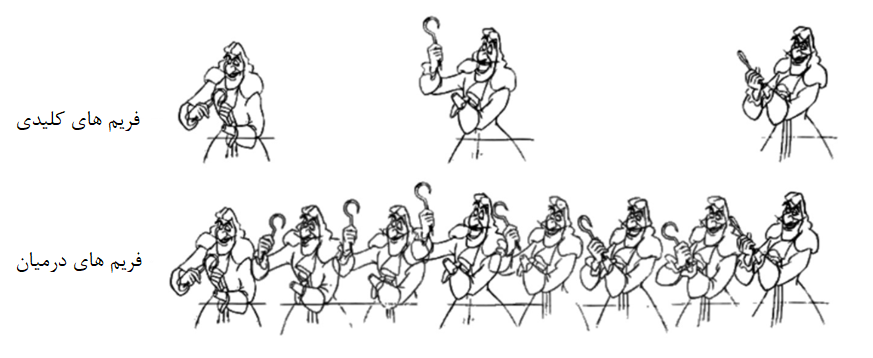
\includegraphics[width=\textwidth,height=\textheight,keepaspectratio]{Figures/Ch1/KeyframeAnimation.png}}

	\caption{فریم‌های کلیدی و درمیان}
	\label{fig:KeyframeAnimation}
\end{figure}

\subsection{چشم‌انداز چندمنظوره}

استفاده از چشم‌انداز چندمنظوره روش دیگری بود که در پویانمایی سنتی استفاده می‌شد.
هماطور که از تصویر زیر مشخص است، برای نمایش یک محیط از یک چشم‌انداز استفاده می‌شد.
این چشم‌انداز می‌توانست نشان دهنده‌ی محیط در فواصل مختلف باشد. در این صورت، زمانی که 
دوربین در صحنه حرکت می‌کرد این توهم را در مخاطب ایجاد می‌کرد که گویی در محیط در حال حرکت هستیم.

\begin{figure}[ht]
	\centerline{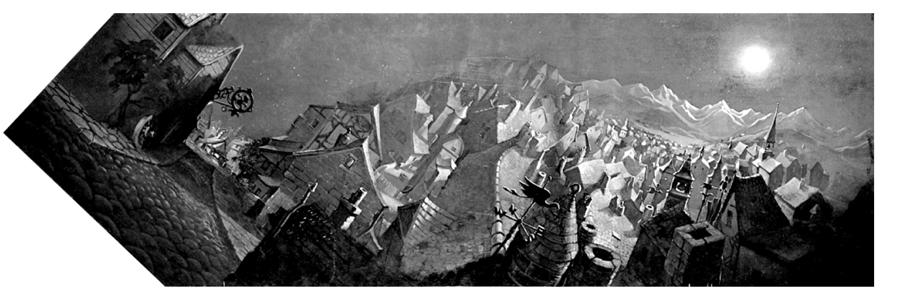
\includegraphics[width=\textwidth,height=\textheight,keepaspectratio]{Figures/Ch1/Panorama.png}}

	\caption{چشم‌انداز چندمنظوره}
	\label{fig:Panorama}
\end{figure}


\subsection{لایه‌های مختلف}

با استفاده از این روش، پویانما‌ها یک صحنه را به چند قسمت مختلف تقسیم می‌کردند.
به صورت مثال لایه‌های مختلف برای هر شخصیت درون صحنه استفاده می‌شد. علاوه برا ین یک لایه نیز برای تصویر پس‌زمینه استفاده می‌شد.
از آنجایی که این لایه‌ها یک صفحه‌ی شفاف بودند بنابراین می‌توان لایه‌‌ها را 
بر روی هم انباشته کرد و با تصویر برداری از بالا تمام صحنه را تصویربرداری کرد.
این روش در تصویر 
\ref{fig:DifferentLayers}
آورده شده است.

\begin{figure}[ht]
	\centerline{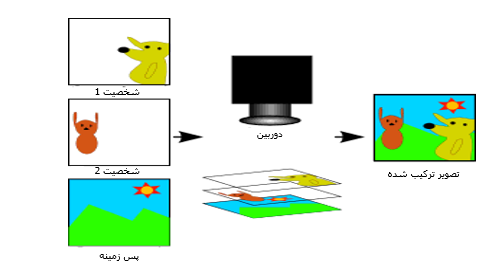
\includegraphics[width=\textwidth,height=\textheight,keepaspectratio]{Figures/Ch1/DifferentLayers.png}}

	\caption{لایه‌های مختلف}
	\label{fig:DifferentLayers}
\end{figure}

\section{پویانمایی کامپیوتری}

اگر بخواهیم نگاهی به تاریخچه‌ی انیمیشن‌های کامپیوتری بیاندازیم، مشاهده می‌کنیم که 
در حدود دهه‌ی 1980 میلادی شرکت دیزنی به عنوان یکی از اولین شرکت‌های جهان، شروع به 
دیجیتالی کردن خط لوله‌ی تولید پویانمایی سنتی خود کرد.
در این دیجیتال‌سازی بسیاری از روش‌ها و ایده‌‌های استفاده شده در پویانمایی سنتی،
به‌کار گرفته‌شد.
اولین مقالات این حوزه توسط آقای جان لستر از کارمندان پیکسار به عنوان 
"اصول پویانمایی سنتی به‌کار رفته در پویانمایی کامپیوتری سه‌بعدی"
ارائه شد.
در این مقاله اصول اولیه پویانمایی سنتی دوبعدی ترسیم شده با دست
و کاربرد آن‌ها در پویانمایی کامپیوتری سه‌بعدی شرح داده شده است.

پویانمایی کامپیوتری تنها محدود به دنیای سینما و فیلم‌های پویانمایی نمی‌شوند و به دنیای
بازی‌های کامپیوتری نیز ورود پیدا کرده‌اند. بازی‌های کامپیوتری سعی می‌کنند دیوار میان تماشاگران و فیلم را بشکنند و 
با تعاملی بودن و دادن آزادی عمل به بازیکن، سعی می‌کنند داستان را به گونه‌ای تعریف کنند که گویی بازیکن یکی از شخصیت‌های اصلی داستان است.
پویانمایی در بازی‌های کامپیوتری اهمیت بسیار بالایی دارد زیرا همانطور که گفته شد باعث 
جان بخشیدن به شخصیت‌ها می‌شود که اهمیت بسیار بالایی برای جلب توجه بازیکنان در هنگام داستان‌سرایی دارد.

با پیشرفت تکنولوژی، همراه با استفاده از روش‌های گذشته، روش‌های جدیدتری برای تولید پویانمایی توسعه یافته‌است که 
در ادامه به چند مورد از آن‌‌ها می‌پردازیم.

\subsection{فریم‌های کلیدی و درمیان}

همانطور که اشاره شد در پویانمایی کامپیوتری از روش‌های موجود در 
پویانمایی سنتی استفاده شده است. در اینجا نیز فریم‌های کلیدی 
یک حرکت توسط پویانماها به وجود می‌‌آیند ولی فریم‌های میانی به جای اینکه توسط پویانماها به وجود آید،
توسط کامپیوتر با استفاده از روش های درون‌یابی به وجود می‌آیند.

\subsection{رویه}

در این روش، حرکت بر اساس یک الگوریتم بیان می‌شود.
درواقع انیمیشن‌ها در این نوع پویانمایی، توابعی با تعداد کمی از متغیر‌ها هستند.
به عنوان مثال یک تابعی را درنظر بگیرید که به گرفتن ورودی ثانیه، دقیقه و ساعت، 
یک شئ ساعت را خروجی دهد که عقربه‌هایش در جای مناسب با توجه به ورودی‌ها قرار گرفته باشد.
حال می‌توان با تغییر ورودی‌ها حرکت ساعت را شبیه‌سازی کنیم.

\subsection{مبتنی بر فیزیک}

پویانمایی مبتنی بر فیزیک پلی میان دنیای پویانمایی با 
دنیای واقعی است. در این روش با نسبت دادن ویژگی‌های فیزیک به اشیاء سه‌بعدی و سپس حل‌کردن
فرمول‌های فیزیک مانند فرمول حرکت یا فرمول‌های نیوتن،
فیزیک را شبیه سازی می‌کند.
پویانمایی‌های مبتنی بر فیزیک شخصیت را قادر می‌سازد تا حرکت‌های خود را 
به صورت پویا با محیط تنظیم کند.

\subsection{ضبط حرکت
\protect \LTRfootnote{Motion Capture}}

به فرآیند ثبت و دیجیتالی‌کردن حرکت یک شئ یا شخص، ضبط حرکت گویند.
ضبط حرکت توسط دوربین‌های مادون قرمز که تعدادی زیادی از آن‌ها در صحنه‌ی ضبط قرار دارند، صورت می‌گیرد.
این دوربین‌ها به صورت شبکه به یکدیگر متصل هستند و پس از کالیبره شدن، آماده‌ی استفاده هستند.
این دوربین‌ها با استفاده از نشانگر‌های سفیدی که بر روی لباس بازیگران 
ضبط حرکت قرار دارد، داده‌های مورد نیازشان را دریافت می‌کنند.
قابل ذکر است این نشانگر‌ها بازتابنده‌ی مادون قرمز هستند.
در نهایت پویانماها به پاکسازی و پردازش این داده‌ها پرداخته تا آن را 
برای استفاده‌ی شخصیت‌های سه بعدی آماده کنند.



\section{موتور بازی‌سازی}
موتور‌های بازی‌سازی پلتفرم‌هایی هستند که ساخت بازی‌های رایانه‌ای را آسان‌تر می‌کنند.
آن ها به شما این امکان را می‌دهند تا عناصر بازی مانند انیمیشن، تعامل با کاربر یا تشخیص برخورد میان اشیاء را در یک واحد ادغام و ترکیب کنید.
\cite{barczak2019comparative}
زمانی که از اصطلاح موتور بازی‌سازی استفاده می‌کنیم منظورمان نرم‌افزارهای قابل توسعه‌ای هستند که می توانند پایه و اساس بسیاری از بازی‌های مختلف باشند.
\cite{GameEngineArchitecture}
موتورهای بازی‌سازی متشکل از اجزای مختلفی هستند که قابلیت‌های لازم برای ساخت بازی را فراهم می‌کنند.
رایج ترین اجزای موتور بازی عبارتند از:
\cite{barczak2019comparative}
\begin{itemize}
    \item[-] مولفه‌ی صدا: نقش اصلی این مولفه تولید جلوه‌های صوتی در بازی است.
    \item[-] موتور رندر: وظیفه اصلی این مولفه تبدیل داده‌های ورودی به پیکسل‌ها، برای به تصویر کشاندن بر روی صفحه است.
    \item[-] مولفه هوش مصنوعی: این مولفه مسئولیت ارائه‌ی تکنیک‌هایی برای تعریف قوانین رفتار شخصیت‌هایی را دارد که توسط بازیکنان کنترل نمی‌شوند.
    \item[-] مولفه انیمیشن: نقش اصلی این مولفه اجرای انیمیشن‌های مختلف مانند حرکت است.
    \item[-] مولفه شبکه: وظیفه اصلی این مولفه قادرساختنِ بازیِ همزمانِ بازیکنان با یکدیگر، از طریق استفاده از دستگاه‌های متصل به اینترنت است.
    \item[-] مولفه منطق یا مکانیک بازی: این مولفه قوانین حاکم بر دنیای مجازی، ویژگی‌های شخصیت‌های بازیکنان، هوش مصنوعی و اشیاء موجود در دنیای مجازی و همچنین وظایف و اهداف بازیکنان را تعریف می‌کند.
    \item[-] ابزارهای نرم‌افزاری: وظیفه اصلی این ابزارها افزایش راندمان و سرعت تولید بازی با موتور بازی‌سازی است. آن‌ها توانایی اضافه‌کردن بسیاری از عناصر مختلف را به بازی‌ها، از انیمیشن و جلوه‌های صوتی گرفته تا الگوریتم‌های هوش مصنوعی، را فراهم می‌کنند.   
\end{itemize}

یکی از مهم‌ترین مولفه‌های موجود در هر موتور بازی، مولفه‌ی انیمیشن آن است. در این پروژه به بررسی سیستم
انیمیشن گراف که وظیفه‌ی پخش انیمیشن‌ شخصیت‌های سه‌بعدی را در موتور بازی آنریل دارد می‌پردازیم.



\section {موتور بازی‌سازی آنریل}

اولین نسل موتور بازی‌سازی آنریل توسط تیم سوینی، بنیانگذار اپیک گیمز
\LTRfootnote {Epic Games}
،
توسعه یافت.
سویینی در سال 1995 شروع به نوشتن این موتور برای تولید بازی‌ تیراندازی اول شخصی به اسم غیرواقعی
\LTRfootnote{Unreal}
کرد.


نسخه‌‌ی دوم موتور بازی‌سازی آنریل در سال 2002 منتشر شد. 

نسخه سوم نیز در سال 2004 پس از حدود 18 ماه توسعه، منتشر شد.
در این نسخه، معماری پایه‌ای موجود در نسخه‌ی اول مانند طراحی شی‌گرا، اسکریپت‌نویسی مبتنی بر داده و رویکرد نسبتا ماژولار نسبت به زیرسیستم‌ها وجود داشت.
اما برخلاف نسخه دوم که از یک خط لوله با عملکرد ثابت
\LTRfootnote{fixed-function pipeline}
استفاده می‌کرد، این نسخه به صورتی طراحی شده بود تا بتوان قسمت‌های سایه‌زنی سخت‌افزاری
\LTRfootnote{shader hardware}
را برنامه‌نویسی کرد.


موتور بازی‌سازی آنریل 4 در سال 2014 در کنفرانس توسعه‌دهندگان بازی
\LTRfootnote{GDC}
منتشر شد.
این نسخه با طرح کسب‌و‌کار اشتراکی برای توسعه‌دهندگان در دسترس قرار گرفت. این اشتراک به صورت ماهانه، با پرداخت 19 دلار آمریکا به توسعه‌دهندگان این اجازه را می‌داد تا به نسخه‌ی کامل موتور، از جمله کد منبع 
\lr {C++}
آن
دسترسی پیدا‌ کنند.
البته در سال 2015 اپیک گیمز موتور بازی‌سازی آنریل را به صورت رایگان برای همگان منتشر ساخت.

آخرین نسخه آنریل به اسم موتور بازی‌سازی آنریل 5 در سال 2020 معرفی شد. این نسخه از تمام سیستم‌های موجود از جمله کنسول‌های نسل بعدی پلی‌استیشن 5
\LTRfootnote{PlayStation 5}
و ایکس‌باکس سری 
\lr{X/S}
\LTRfootnote{Xbox Series X/S}
پشتیبانی می کند.
کار بر روی این موتور حدود دو سال قبل از معرفی آن شروع شده بود. در سال 2021 نسخه‌ای از آن به صورت دسترسی اولیه منتشر شد. به طور رسمی در سال 2022 نسخه‌ی کامل این موتور برای توسعه‌دهندگان انتشار یافت.
\cite{UnrealEngineWikiPedia}
